\PassOptionsToPackage{unicode}{hyperref}
\documentclass[
  ukrainian,
  14pt
]{extreport}
\usepackage{lmodern}
\usepackage{hyperref}
\makeatletter
\hypersetup{
    colorlinks=true,
    linkcolor=blue,
    filecolor=magenta,
    urlcolor=cyan,
}
\makeatother
\usepackage{amssymb,amsmath,amsthm,url}
\usepackage[margin=2cm]{geometry}
\usepackage{longtable,booktabs}
\usepackage{etoolbox}
\usepackage{titling}
\usepackage{graphicx}
\usepackage{float}
\usepackage[dvipsnames]{xcolor}
\usepackage[ukrainian]{babel}
\usepackage{setspace}
\usepackage{xcolor}
\usepackage{multirow}
\usepackage{comment}
\usepackage{booktabs}
\usepackage{tikz}
\setcounter{secnumdepth}{-1} 
\usepackage{unicode-math}
  \defaultfontfeatures{Scale=MatchLowercase}
  \defaultfontfeatures[\rmfamily]{Ligatures=TeX,Scale=1}
  \setmainfont[]{Times New Roman}
  \setsansfont[]{Arial}
  \setmonofont[]{Consolas}
  \makeatother
\usepackage[labelsep=period]{caption}
\usepackage{subcaption}

\author{}
\title{\Huge Лабораторна робота №5 \\\Large ПОБУДОВА ПІДСИЛЮВАЛЬНИХ КАСКАДІВ НА
ТРАНЗИСТОРАХ}
\date{}
             
\begin{document}
\begin{titlepage} 
	\newcommand{\HRule}{\rule{\linewidth}{0.5mm}} 
	
	\center 
	
	\textsc{\Large МІНІСТЕРСТВО ОСВІТИ І НАУКИ УКРАЇНИ\\ \Large КИЇВСЬКИЙ НАЦІОНАЛЬНИЙ УНІВЕРСИТЕТ ІМЕНІ ТАРАСА ШЕВЧЕНКА}\\[1.5cm] 

	
	\HRule\\[0.4cm]
	
	{\huge \bfseries  Лабораторна робота №5 \\\Large \bfseries 
  Побудова підсилювальних каскадів на транзисторах
    }\\[0.4cm]
	
	\HRule\\[1.5cm]

	
	

	{\large\textit{Автор}}\\
	\large Столяров Андрій Дмитрович, \\\large група 5-А, Фізичний Факультет 
	
	
	\vfill\vfill\vfill 
	\vfill
	{\normalsize Київ, \today} 
\end{titlepage}
\tableofcontents
\clearpage
\section{Вступ}
Об'єктом дослідження є емітерний повторювач, парафазний, диференціальний
підсилювач та підсилювач зі спільним емітером.
Предмет дослідження: теоретичні основи, принципи роботи, фізичний зміст і
застосування підсилювачів.
\subsection{Мета}
Виміряти коефіцієнти передачі за напругою підсилювальних
каскадів різних типів для гармонічних і імпульсних вхідних сигналів, а також зсуви
фаз між вихідними і вхідними сигналами. 
\subsection{Методи дослідження}
Одночасне спостереження вхідного та вихідного сигналів
на екрані двоканального осцилографа із наступним вимірюванням і порівнянням їх
параметрів 
\section{Теоретичні відомості}
\textbf{Підсилювач електричних сигналів} – радіоелектронний пристрій, що
перетворює вхідний електричний сигнал, який являє собою залежність від часу
напруги $U_{\text{вх(t)}}$ або струму $I_{\text{вх(t)}}$, у пропорційний йому вихідний сигнал $U_{\text{вих(t)}}$ або
$I_{\text{вих(t)}}$, потужність якого перевищує потужність вхідного сигналу. Будь-який
підсилювач електричних сигналів можна розглядати як активний чотириполюсник,
маючи змогу досліджувати частотні характеристики підсилювача (його відгук на
гармонічний сигнал певної частоти), імпульсні характеристики (відгук на
одиничний імпульсний сигнал у вигляді $\delta$-функції) або перехідні характеристики
(відгук на ступінчасту зміну вхідного сигналу).
\textbf{Підсилювальний каскад} – підсилювач, який містить мінімальне число
підсилювальних елементів (1–2 транзистори) і може входити до складу
\textit{багатокаскадного підсилювача.}
\textbf{Коефіцієнт передачі за напругою} — відношення амплітуди вихідного
напруги підсилювача до амплітуди вхідної
\textbf{Класифікація, будова та принцип роботи транзисторів}
Будь-який підсилювач електричних сигналів можна розглядати як
активний чотириполюсник. Проходження сигналу через такий
чотириполюсник можна розглядати за допомогою тих самих методів, які
застосовувались для пасивних чотириполюсників. Зокрема, вхідний сигнал
можна подавати як суперпозицію гармонічних сигналів (спектральний
метод), у вигляді суми коротких імпульсів або як суперпозицію стрибків
сигналу. Відповідно можна досліджувати частотні характеристики
підсилювача (його відгук на гармонічний сигнал певної частоти), імпульсні
характеристики (відгук на одиничний імпульсний сигнал у вигляді -
функції) або перехідні характеристики (відгук на ступінчасту зміну
вхідного сигналу). Всі ці характеристики взаємопов’язані і знаючи одну з
них, можна одержати інші.
Найширше використовується спектральний метод. На кожній частоті
підсилювач можна охарактеризувати такими параметрами, як основна
передавальна функція (коефіцієнт передачі) $\tilde{K}(w)$ (у загальному випадку
комплексна) та вхідний і вихідний комплексні опори $ \tilde{Z}_{in} (w)$ і $\tilde{Z}_{out} (w)$
відповідно.
Коефіцієнтом передачі за напругою називають відношення напруг сигналів
на виході і на вході підсилювача:
$$
\widetilde{K}_{u}(w)=\frac{\widetilde{U}_{\text {out }}(w)}{\widetilde{U}_{\text {in }}(w)}=K_{u}(w) e^{i \varphi(w)}
$$
Цю залежність називають частотною характеристикою підсилювача. При
цьому залежність $K_u(w)$ називається амплітудно-частотною
характеристикою (АЧХ), а залежність $\varphi(w)$ — фазо-частотною
характеристикою (ФЧХ) підсилювача.

\section{Хід Роботи}
\subsection{Емітерний повторювач}
\begin{figure}[H]
  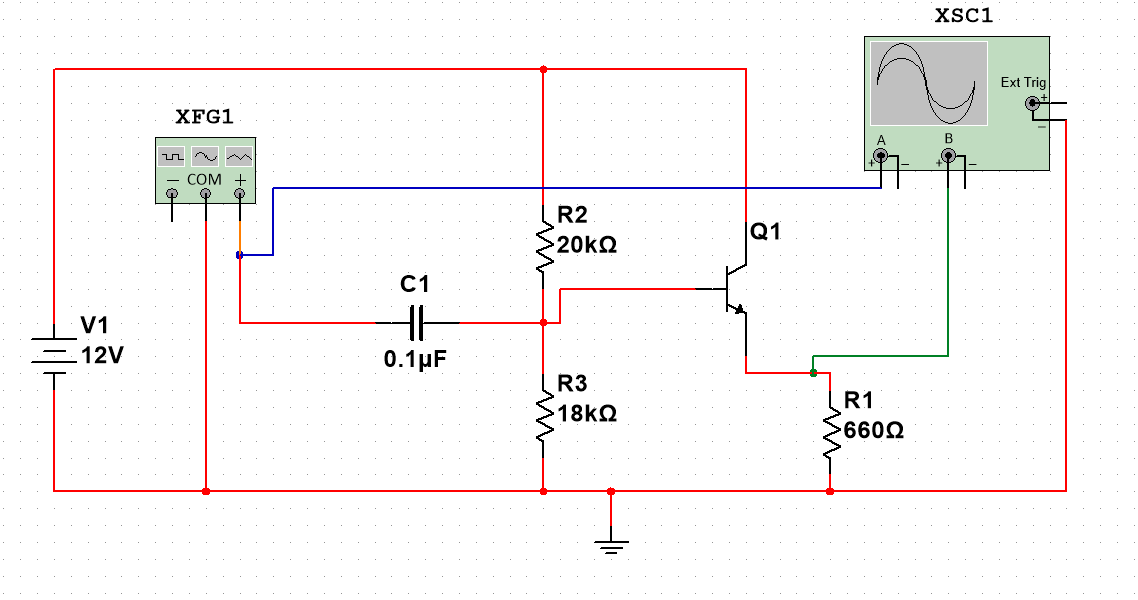
\includegraphics[width=0.7\textwidth]{imgs/1-1.png}
  \centering
  \caption{Схема}
\end{figure}
\begin{figure}[H]
  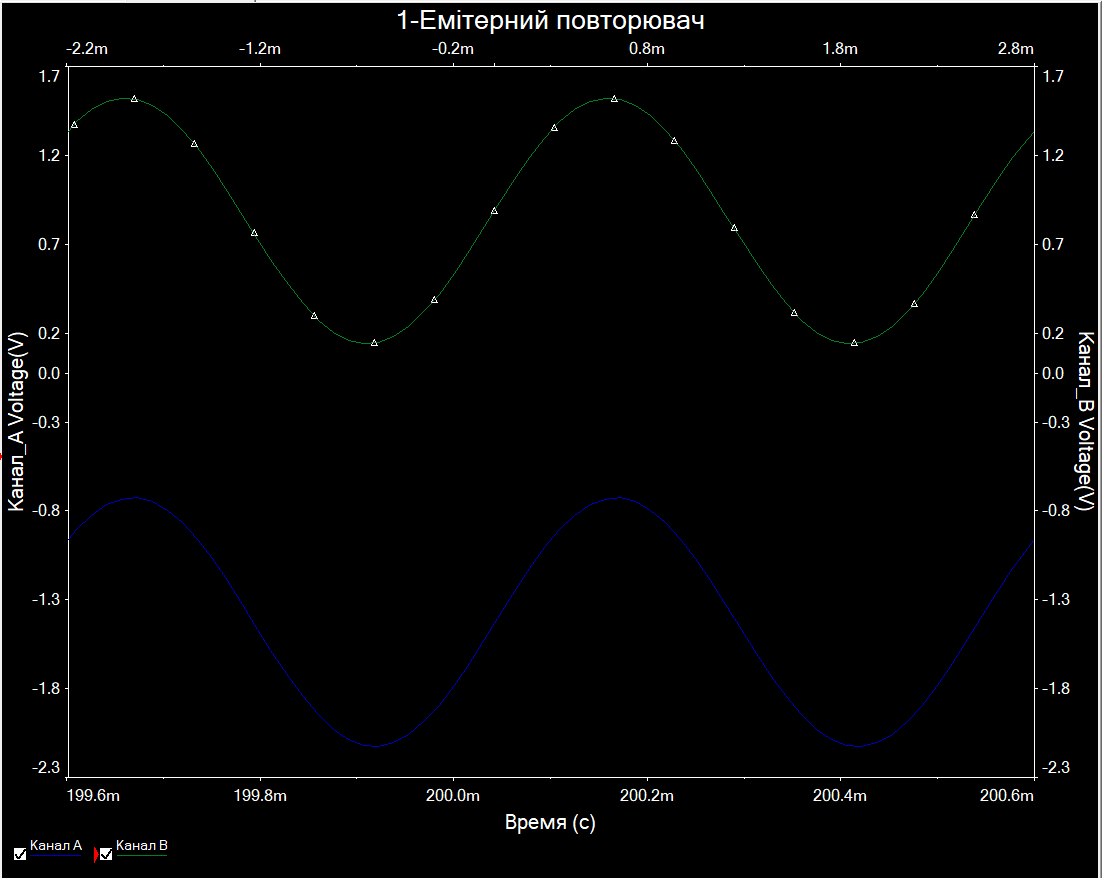
\includegraphics[width=0.7\textwidth]{imgs/1-2.png}
  \centering
  \caption{Графік залежності вхідного та вихідного сигналу емітерного підсилювача від часу.
  }
\end{figure}

\subsection{Парафазний підсилювач}
\begin{figure}[H]
  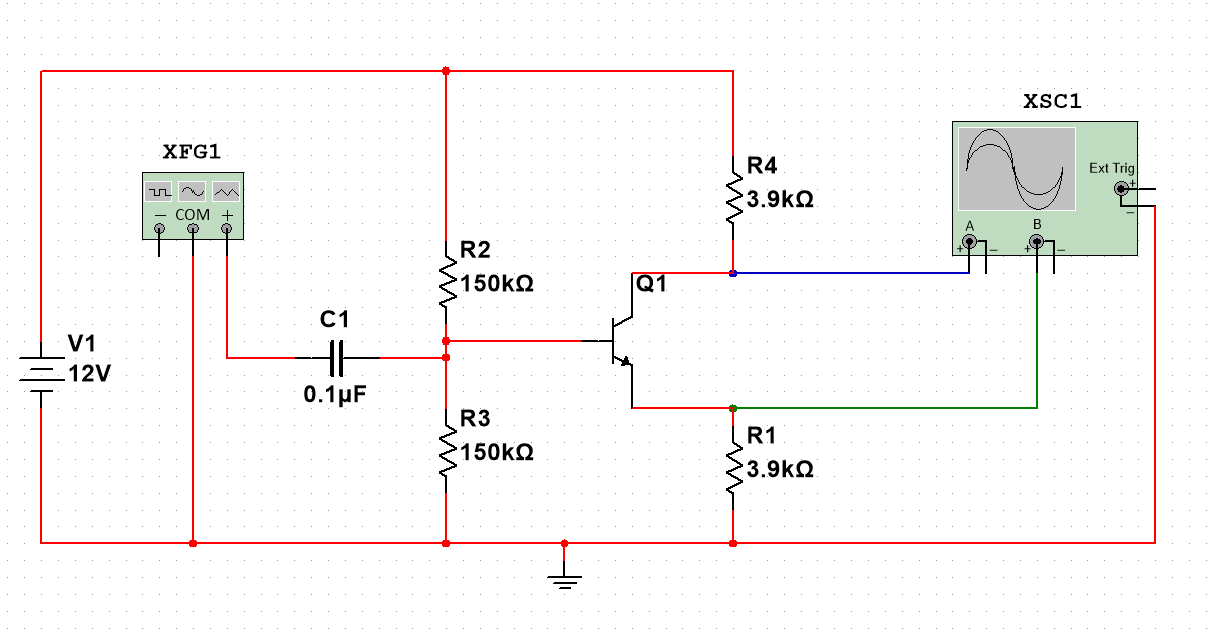
\includegraphics[width=0.7\textwidth]{imgs/2-1.png}
  \centering
  \caption{Схема}
\end{figure}
\begin{figure}[H]
  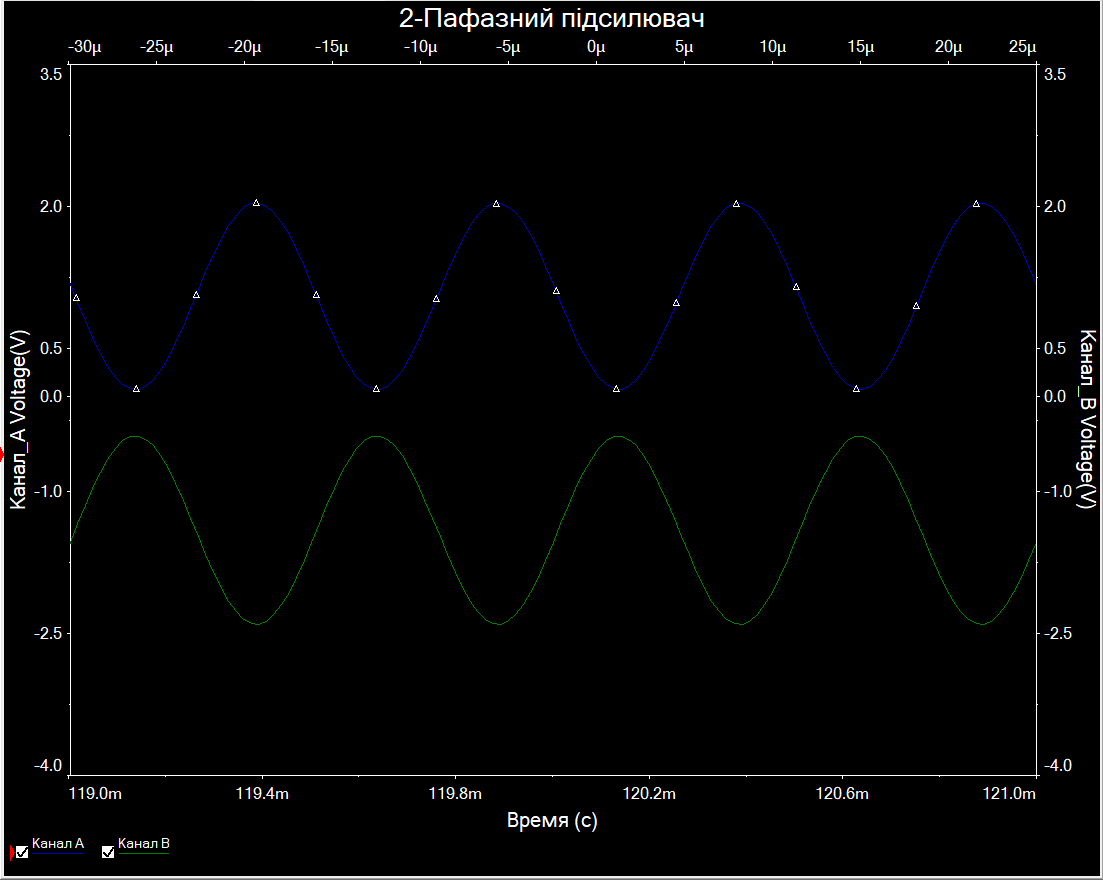
\includegraphics[width=0.7\textwidth]{imgs/2-2.png}
  \centering
  \caption{Графік залежності вхідного та вихідного сигналу від часу.
  }
\end{figure}

\subsection{Підсилювач зі спільним емітером.}
\begin{figure}[H]
  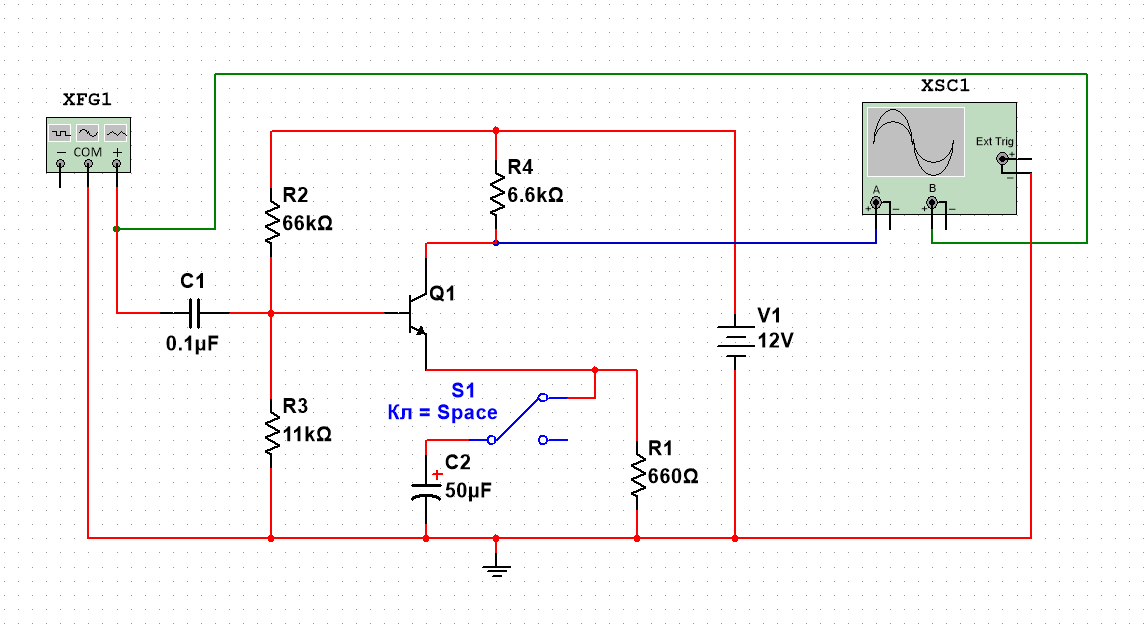
\includegraphics[width=0.7\textwidth]{imgs/3-1.png}
  \centering
  \caption{Схема}
\end{figure}
\begin{figure}[H]
  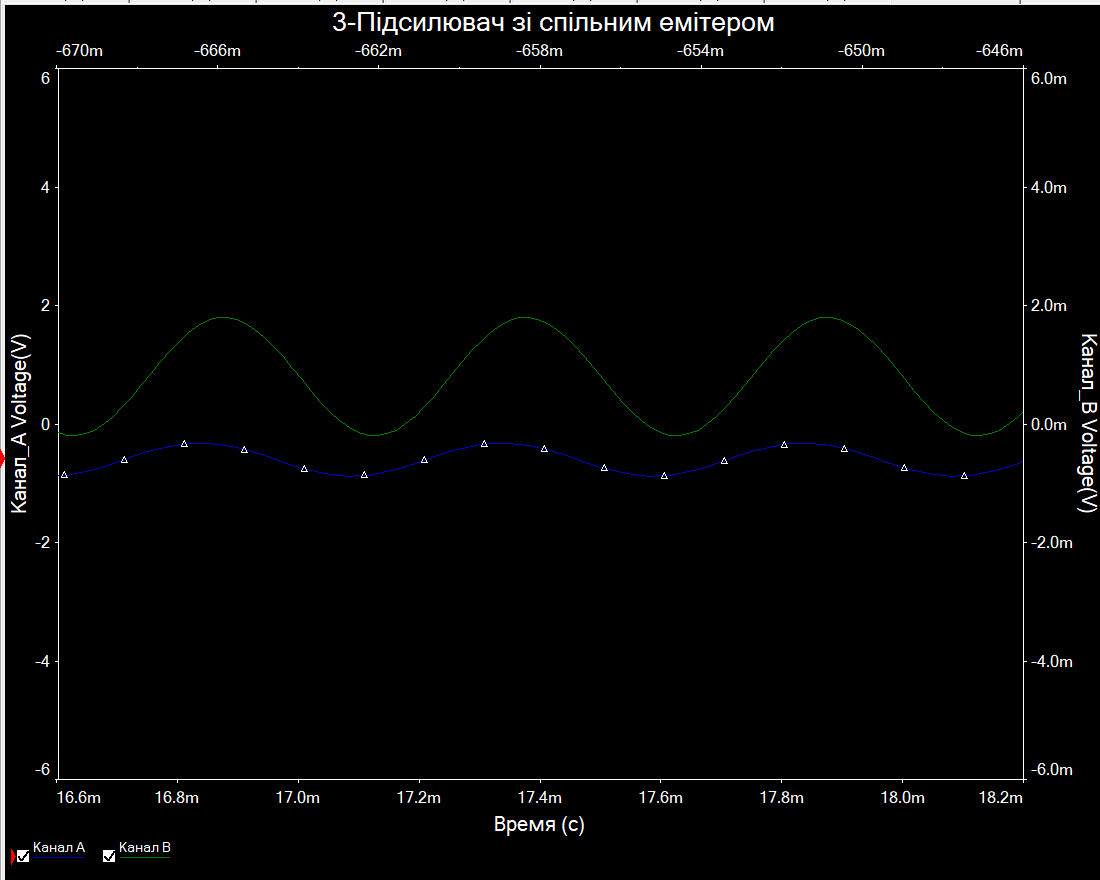
\includegraphics[width=0.7\textwidth]{imgs/3-2.png}
  \centering
  \caption{Графік залежності вхідного та вихідного сигналу від часу.
  }
\end{figure}
\begin{figure}[H]
  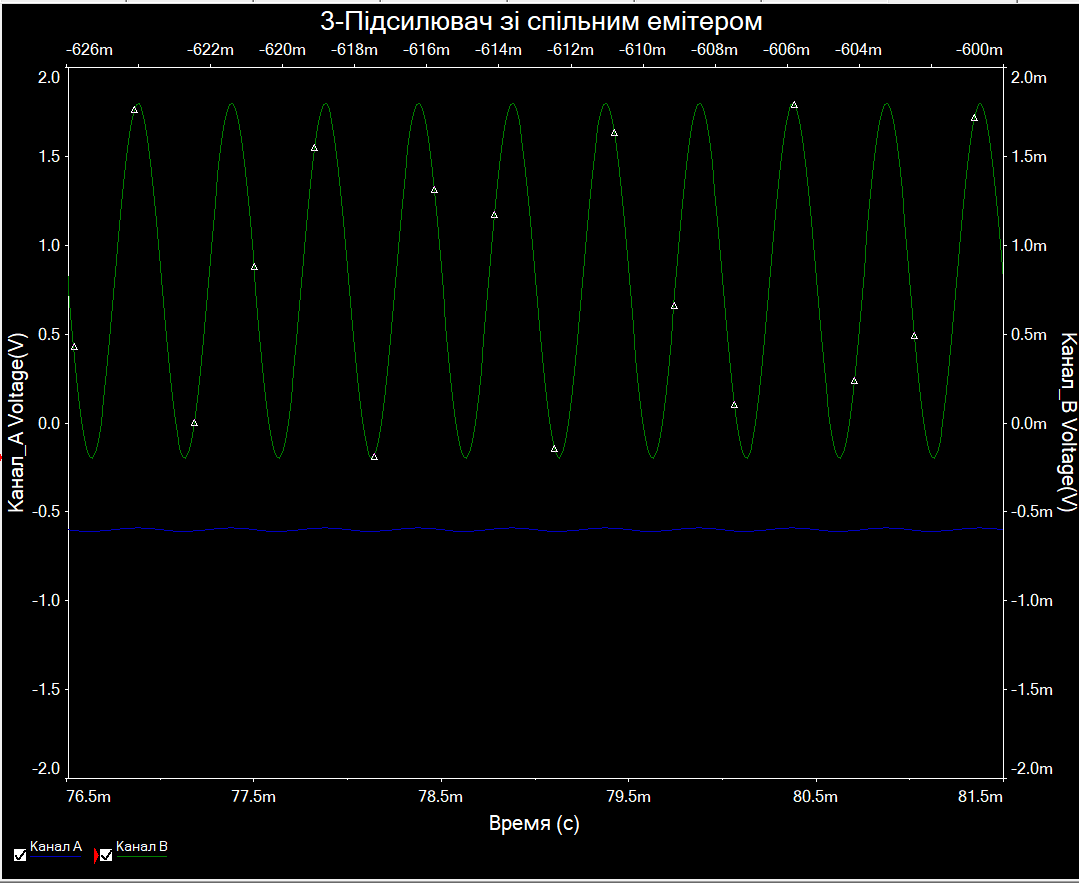
\includegraphics[width=0.7\textwidth]{imgs/3-3.png}
  \centering
  \caption{Графік залежності вхідного та вихідного сигналу від часу.(з конденсатором)
  }
\end{figure}

\subsection{Диференціальний підсилювач}
\begin{figure}[H]
  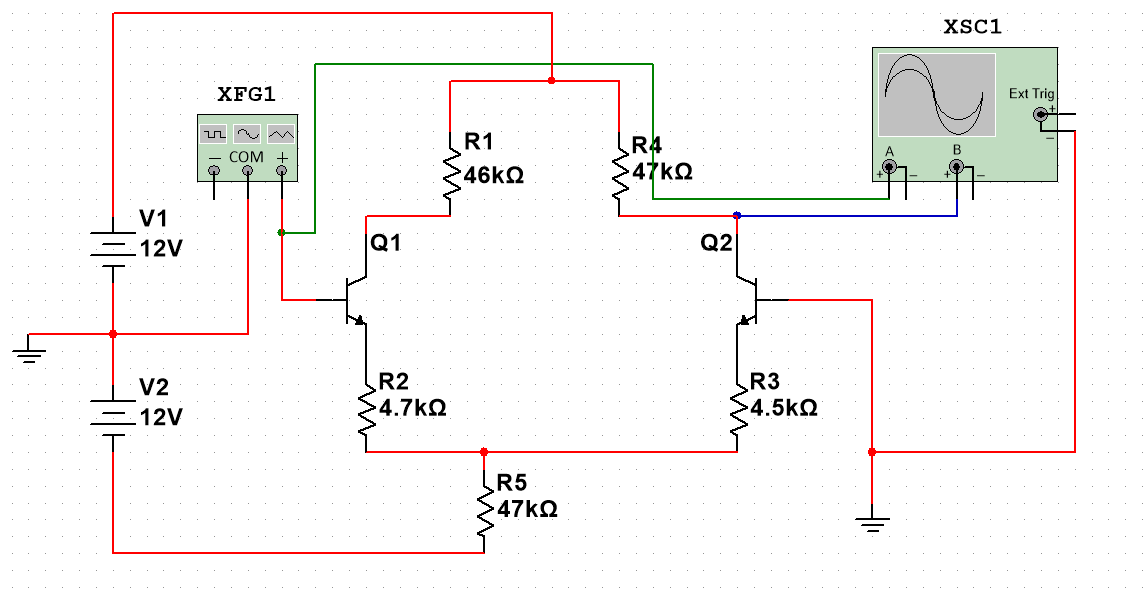
\includegraphics[width=0.7\textwidth]{imgs/4-1.png}
  \centering
  \caption{Схема}
\end{figure}
\begin{figure}[H]
  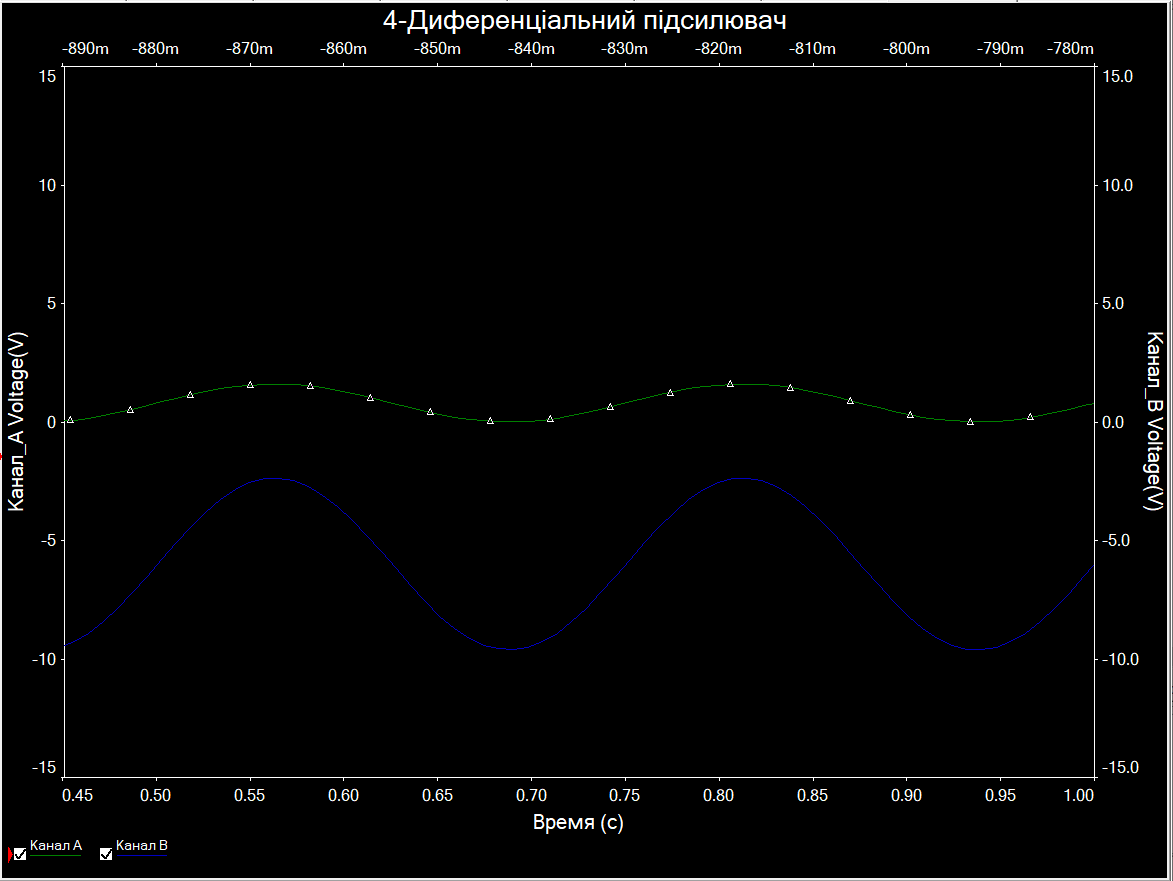
\includegraphics[width=0.7\textwidth]{imgs/4-2.png}
  \centering
  \caption{Графік залежності вхідного та вихідного сигналу від часу.
  }
\end{figure}

\subsection{Cинфазний диференціальний підсилювач}
\begin{figure}[H]
  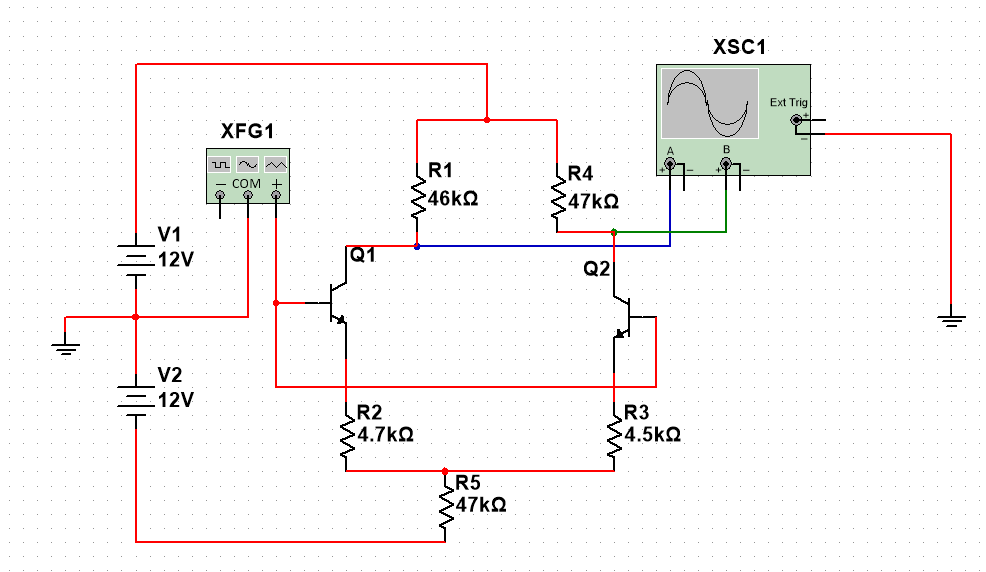
\includegraphics[width=0.7\textwidth]{imgs/5-1.png}
  \centering
  \caption{Схема}
\end{figure}
\begin{figure}[H]
  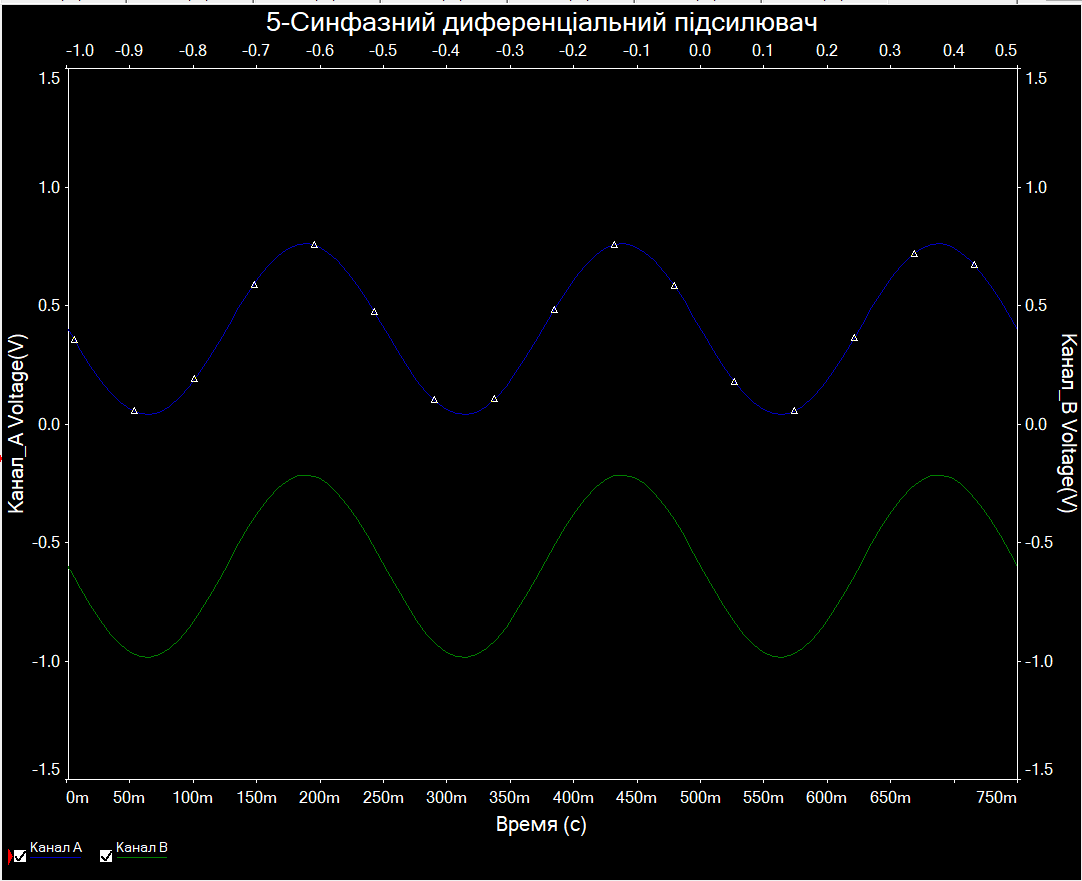
\includegraphics[width=0.7\textwidth]{imgs/5-2.png}
  \centering
  \caption{Графік залежності вхідного та вихідного сигналу від часу.
  }
\end{figure}
\section{Висновок}
У цій лабораторній роботі я ознайомився з тим як змінюється сигнал
після проходження через підсилювальні каскади різних типів за допомогою
методу співставлення. Робота проводилась із емітерним повторювачем,
пафазним підсилювачем, підсилювачем зі спільним емітером,
диференційним та диференційним синфазним підсилювачами, в результаті
отримав зображення змінених сигналів, які повністю збігаються із
очікуваними. Залежності вхідних та вихідних сигналів від часу є хорошими
демонстраціями відмінностей досліджуваних підсилювачів. Порівнявши їх, можна
зрозуміли принцип роботи кожного підсилювача.

Робота виконувалась у програмі \textbf{Multisim14}.
\end{document}